\Chapter{Komponensek}
\label{Chap:komponensek}

\section{Felhasznált technológiák}

% C++, SDL

Windows operációs rendszeren az egyik legnépszerűbb integrált fejlesztőkörnyezet a Microsoft Visual Studio, aminek a 2015-ös verzióját használom. Ennek felülete a fejlesztők számára egyszerűen áttekinthető, kényelmesen elérhetővé teszi a szükséges funkciókat. A játék megírásához a C++ programozási nyelv tűnt a legmegfelelőbbnek. A mai játékok jó részét szintén ezen a nyelven írják, mivel a fordítást követően natívan fut a program. A játékok esetében általában hatékonyabb erőforráskihasználást tesz lehetővé.

A képi világ kirajzolásához, illetve a hangok megszólaltatásához az SDL 2.0-t választottam. Az alábbi linken található bővebb leírás, hogy mit is takar pontosan az SDL \cite{SDL}.

% TODO: Itt is kellene kicsit részletezni, hogy mi található a linken!
Ez egy olyan alkalmazás, vagy játékfejlesztési segédeszköz, amelynek komponenseit felhasználva platformfüggetlenül lefordítható a forráskód. Működik Linux-on, Windows-on, MacOSX-en, illetve bármely egyéb operációs rendszeren.

\section{Az alkalmazás fő részei}

A fő részek, és azok kapcsolatainak szemléltetéséhez egy osztálydiagramot készítettem (\ref{fig:uml} ábra.). Ezen megtekinthető a játék felépítése, melyik osztálynak melyik az őse, illetve mely osztályok vannak kapcsolatban egymással. Továbbá feltüntetésre kerültek a kapcsolatokhoz szükséges adattagok, metódusok.

A \texttt{MainGame} a játék fő osztálya. Ehhez kapcsolódik minden egyéb komponens, és ez felel az ablak inicializálásáért, felhasználói interakciók kezeléséért. A játékbeli interakciók kezeléséért az \texttt{Action} osztály felelős, ez kezeli az állapotokat, például hogy éppen előre vagy hátra haladunk, ugrunk, vagy futunk. Ennek megfelelően az \texttt{Action} osztály kimenetei alapján a \texttt{Player} osztály végzi el a játékoshoz kapcsolódó cselekvéseket. A \texttt{MainGame}-hez kapcsolódik még közvetlen a \texttt{Map}, a \texttt{Sound}, a \texttt{MainMenu} osztály. 

A \texttt{Map} a játéktér elemeit, és az azokhoz kapcsolódó objektumokat fogja össze. Ide kapcsolódik a \texttt{HeightMapDrawer}, amin keresztül betölti, kirajzolja a játék alapját képző domborzatot, és kiszámolja a karakter ütközésvizsgálatához szükséges gradienst is. A \texttt{VboDrawer} és őse, a \texttt{ModelLoader} az egyéb játékbeli objektumok (fák, tárgyak) betöltéséért, kirajzolásáért felelős. A \texttt{BulletCalcs3D} a lövéshez kapcsolódó háttérszámításokat végzi, és az adott háromszöggel kapcsolatos x,y,z metszéspontot adja vissza. A \texttt{Materials} osztály az anyagjellemzők beállításáért felelős.

A játék részét képezik a játékos informálásáért és segítéséért felelős 2D-s elemek is, amelyekért az \texttt{IngameElements2D} osztály felelős. Ez jeleníti meg a célkeresztet, rajzolja ki az életerő és a lőszer mennyiséget jelző textúrát is, amelyeket viszont a \texttt{Texture} osztály tölt be.

A \texttt{MainMenu} osztályban a főmenühöz kapcsolódó elemek vannak, amelyek a menü háttere, illetve a kijelölések lekezelése vizuálisan. Ezeket az elemeket is a \texttt{VboDrawer} és őse a \texttt{ModelLoader} tölti be, rajzolja ki.

A \texttt{Sound} a hangok megszólalásáért, a megfelelő zenék lejátszásáért felelős, az \texttt{Utils} pedig az egyéb, többi osztályba nem tartozó elemeket tartalmazza.

\begin{figure}[h]
\centering
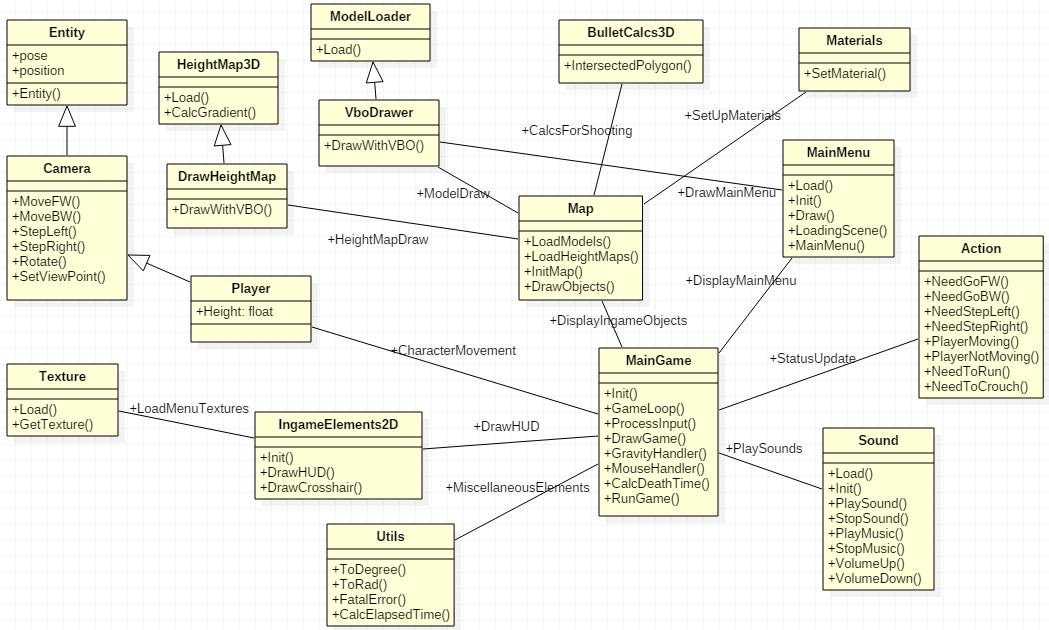
\includegraphics[scale=0.5]{kepek/uml.png}
\caption{A játék felépítése}
\label{fig:uml}
\end{figure}

\subsection{Magasságmező betöltése, textúrázása}

A játék \texttt{.obj} kiterjesztésű modelleket használ, és ezekre húzza rá a textúrát. A megjelenítéshez VBO-t, azaz \textit{Vertex Buffer Object}-et használ, ami a modell adatait tárolja, és egyben, a legmegfelelőbb formátumban adja át a videókártyának.

Ez egy fekete fehér kép 256 színárnyalatából tud 256 különböző magasságértéket számolni. A fekete a legalacsonyabb, a fehér a legmagasabb terület, így könnyedén lehet hegyeket illetve völgyeket kialakítani. A játék játszható területének megadásához például \aref{fig:heightmap} ábrán látható képet adhatjuk meg, amiből a program a magasságértékeket számolja. A magasságmező textúráját egy külön képfájlból tölthetjük be. Egy ilyen látható \aref{fig:heightmap_texture} ábrán.

\begin{figure}[h]
\centering
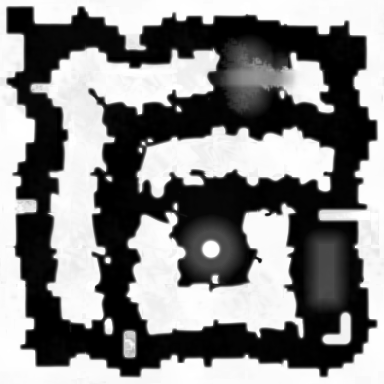
\includegraphics[scale=0.5]{kepek/heightmap.png}
\caption{A magasságmező adatait tartalmazó bitmap}
\label{fig:heightmap}
\end{figure}

\begin{figure}[h]
\centering
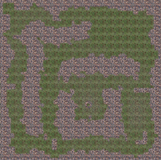
\includegraphics[scale=1.5]{kepek/heightmap_texture.png}
\caption{A magasságmező textúrája}
\label{fig:heightmap_texture}
\end{figure}

\Aref{fig:screenshot} képen pedig a játékban való megjelenés látható. A magasságmező használata abból a szempontból is előnyös, hogy egyszerűen megoldható vele a függőleges irányú ütközésvizsgálat, illetve az egyes részek meredekségéből közvetlenül kiszámíthatóak a bejárható területek. A magasságmező pontokból való előállításához az egyik legegyszerűbb megoldást a lineáris interpoláció adta. A textúra illesztése a nagy abszolút értékű gradiensek esetében problémás. Erre megoldást például a multitextúrázás jelenthet.

\begin{figure}[h]
\centering
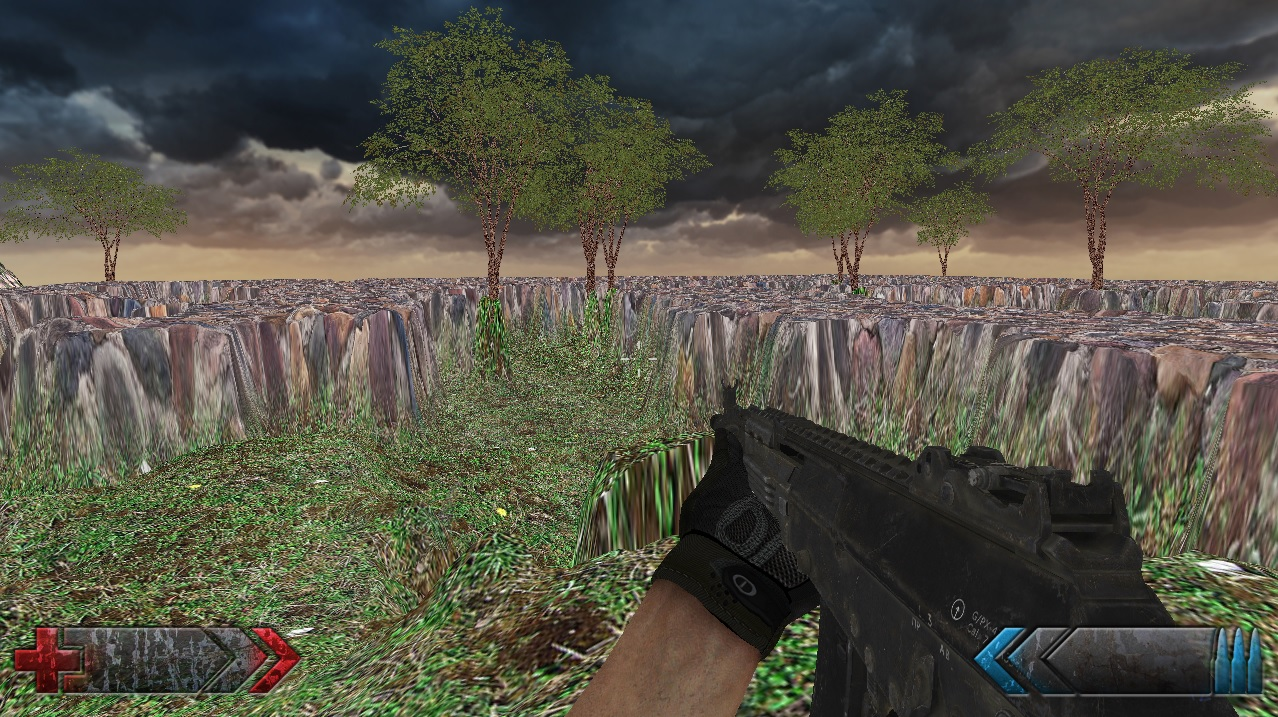
\includegraphics[scale=0.4]{kepek/screenshot.png}
\caption{A megjelenített magasságmező}
\label{fig:screenshot}
\end{figure}

\subsection{A karakter irányítása és a játék fizikája}

A játékban egy karaktert irányíthatunk az ő szemszögéből. A karakternek van magassága, térbeli pozíciója, nézési iránya. A nézeti iránynak megfelelő térrészt láthatjuk a játékos szemszögéből. A látható térrész alsó részén látszik a karakterhez tartozó fegyver, illetve annak a keze.

% TODO: Ezt az irányítás megvalósításánál kellene megemlíteni.

% A kamerához van forgatva a fegyvere, és az ő szemszögéből látható testrészei. Minden cselekedetéhez tartozik egy bool (két állapotú) változó. Például ha tegyük fel előre megyünk, akkor az ehhez tartozó változó „true (igaz)” értéket vesz fel, amelyhez különböző eseményeket lehet kötni, mint például a kamera előre mozgatását, bizonyos animációk lejátszását. Továbbá a játékosra folyamatosan hat egy gravitációs erő, ami egy float típusú szám. Ezzel lehet elérni azt, hogy ha ugrunk, a játékos visszaessen a talajra.

\subsection{Hangok betöltése és lejátszása}

Egyidejűleg több hang lejátszására is szükség lehet, amelyet valamilyen események váltanak ki. A karakter előrehaladása közben egyidejűleg ha lövünk, az már több hangcsatornát igényel. Ha csak egy csatorna lenne, akkor a lépéshang lejátszása után, vagy azt megszakítva lehetne csak lejátszani a lövés hangját. A játék alatti zenéhez szintén szükséges egy külön csatorna.

\begin{figure}[h]
\centering
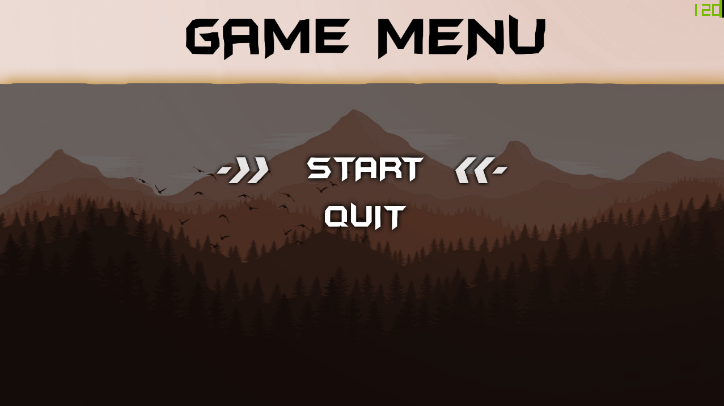
\includegraphics[scale=1.6]{kepek/menu.png}
\caption{A főmenü}
\label{fig:menu}
\end{figure}

\begin{figure}[h]
\centering
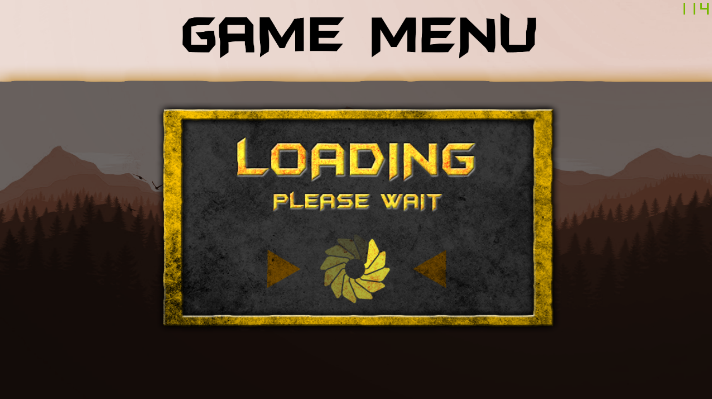
\includegraphics[scale=1.6]{kepek/loading_screen.png}
\caption{Pályabetöltés közben ez látható}
\label{fig:loading}
\end{figure}

\subsection{Lövéssel kapcsolatos számítások}

A lövés háttérszámításait egy külön komponens végzi. A számítások elvégzésére minden képkocka renderelése előtt szükség van. Ennek első lépése, hogy kiszámítjuk azt a vektort, amerre a játékos néz. Mivel a világ háromszögekből épül fel, ezért ki kell számolni az egyenes háromszöggel való metszéspontját. Bemeneti adatként tehát a játékteret alkotó háromszögek vannak benne, a játékos irányvektor, kimenetként pedig azon $(x, y, z)$ koordinátákat várjuk, amely pontban az ütközés bekövetkezett, illetve plusz információnként a metszett objektumot is tudnunk kell azonosítani. Több százezer háromszögről beszélünk, ezért ez további optimalizálandó problémákat vet fel, amit a későbbiekben mutat be részletesen a dolgozat.

\subsection{Mesterséges intelligencia}

Mivel nem egy elsősorban online játszható, FPS játékról van szó, így mindenképpen szükséges egy, az ellenfelek mozgását irányító mesterséges intelligencia. Az ellenfelek mozgásához az útvonalak keresése A* algoritmus segítségével történik. A játék véletlenszerűen, különböző helyekre kirak adott mennyiségű ellenfelet, amiknek közeledni kell a játékos felé, különböző kritériumoknak megfelelve. Ezek a kritériumok azért kellenek, mert a pályán vannak játékelemek, amiken nem lehet átmenni, illetve az ellenfelek sem mehetnek egymásba. 

Az alapötlet az, hogy a pályán le lesznek rakva pontok (úgynevezett \textit{waypointok}), amelyek csak az ellenfelek számára lesznek láthatók. Ha kikerül egy adott ellenfél a pályára, az első feladata az lesz, hogy megkeresse a hozzá legközelebb eső waypointot. Ezután az A* algoritmus segítségével meghatározza a játékoshoz legközelebb eső waypointhoz vezető legrövidebb utat, végigmegy rajta, majd ha elérte, akkor onnantól a játékos lesz a közvetlen elsődleges célpontja. Mivel a játékos folyamatosan mozog, mindezt másodpercenként legalább 15-30x kell kiszámolni.

Bemeneti adatként a waypointok állnak rendelkezésre, kimenetként pedig az útvonalat várjuk, amerre az ellenfelek mozogni szeretnének. Az ellenfél elsődleges célpontja a játékos, de adódhatnak olyan helyzetek amikor előtte egyéb dolgokat helyez előtérbe, mint például az életerő töltés, vagy lőszer felvétel. Itt fontos szerepet kap az ellenfél karakterisztikája, ami szintén bemeneti paraméter.

\section{A játékindítás folyamata}

A játék indításának folyamata \aref{fig:starting}. ábrán látható.

Első lépésben a játék létrehozza az SDL ablakot, és konkrétan beállítja annak pozícióját, függőleges és vízszintes felbontását, a teljes képernyős módot, illetve elrejti az egérkurzort.

A második lépés hogy az előtte létrehozott ablakot beállítja aktívra, és OpenGL megjelenítésre. Létre kell hozni egy érvényes OpenGL kirajzolás kontextust, hogy inicializáljuk a belépési pontokat. Ez használhatóvá teszi az összes elérhető funkciót, amit az OpenGL magban definiáltak. Ezután betölti a főmenü megjelenítéséhez szükséges modelleket, textúrákat.

Harmadik lépésben aktiválja a hangok megszólaltatásáért felelős komponenst, és betölti az összes hangot, zenét.

A negyedik lépésben aktiválja az eseménykezelő komponenst, ami a felhasználótól érkező interakciókat kezeli, majd meghívja a betöltött modelleket kirajzolásra.

A menübe érkezés után a felhasználónak lehetősége nyílik a játékteret betölteni, vagy kilépni. 

A „Start” gombra kattintás után, betöltődik a magasságmező kezelő komponens, a kamera a kezdőpontra pozícionálódik, elkezdődnek a játékmenethez elengedhetetlen háttérszámítások, és egy új zene lejátszása, betöltődnek a játéktér modelljei, elemei, illetve átvált azok kirajzolására. Hogy a játékos informálva legyen, ez idő alatt megjelenik a betöltőképernyő.

\begin{figure}[h]
\centering
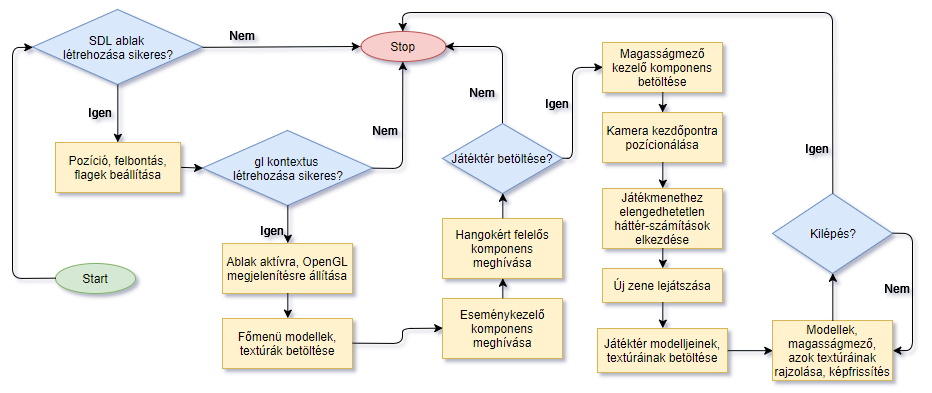
\includegraphics[scale=0.46]{kepek/starting_diagram.png}
\caption{A játék indításának folyamatábrája}
\label{fig:starting}
\end{figure}

